\chapter{The Current State of Technical Recruitment}

This chapter examines the operational framework of modern technical hiring to identify the systemic inefficiencies that necessitate a multimodal screening approach.
The chapter begins by exploring the diversities inherent in technical roles as well as the limitations of job descriptions as a formal, yet inconsistent, role specification.
Following this, the chapter outlines the standard multi-stage recruitment process pipeline and evaluates the various data sources that are typically leveraged during candidate screening.
The discussion concludes by investigating traditional manual screening, as well as the specific challenges faced due to various cognitive biases as well as fatigue.
By establishing these foundational elements, this chapter demonstrates that a reliance on the Curriculum Vitae as a single source of truth is insufficient for technical selection.
This identifies a critical need for automated solutions, and the technical frameworks explored in the subsequent chapter ultimately justify the need for MERIT as a multi-source solution for verifiable candidate assessment.

\section{Technical Roles}

Technical roles refer to those within the technology sector. They often vary in terms of the competencies required and
also span many different domains, from full-stack development to cloud infrastructure management, to machine learning.
In most cases, these roles are listed under generic titles, such as ``Software Engineer'', while the competency and seniority
for the role differ drastically between vacancies. Due to this, it is likely that candidates from adjacent domains may
apply for the same role, even if they are not a good fit. This ambiguity warrants a job description to specify the
competencies and seniority expected for each vacancy.

\section{Job Description}

A job description (JD) is a document that outlines the purpose of a role, as well as the competencies required.
In the technical landscape, requirements are usually explicitly listed, such as programming languages, frameworks,
tooling, seniority and responsibilities. Hiring managers use this text to decide which skills to prioritise,
and to what extent each of these should influence shortlisting, however, most JDs are written for candidates,
not for machines. As such, there is often prose that is not relevant to the screening process, such as benefits and company culture.

There is currently no industry standard for JDs, hence they differ in terms of clarity and depth.
Some postings detail requirements precisely, while others follow boilerplate text that repeats common terms across roles.
Candidates often form unrealistic expectations due to this lack of clarity and specificity \cite{breaugh1983,earnest2011}. 

Regardless, in most cases, the JD can be seen as a valuable source of information for the screening process, given that
the system is able to separate the requirements from the prose. Many screening systems do not take advantage of this, instead
applying fixed weights and metrics to measure against, even when the JD may vary in terms of stack and seniority level~\cite{gugnani2020,lo2025aihiring}.
A screening system that is not tailored to a specific JD is likely to be generic, and may pick the best ``average'' candidate,
rather than the best candidate for that specific role. Given this, rigid scoring systems may miss strong candidates, and
shortlist candidates that are not a good fit for the role when the screening configuration does not reflect the JD~\cite{fuller2021hiddenworkers}

MERIT must, therefore, treat the JD as a noisy configuration document, separating explicit requirements from redundant
information. It extracts listed technical metrics and suggests relative weights via corpus-aware TF-IDF, which recruiters
can add to, remove or override before scoring.

\section{Recruitment Process Pipeline}

Figure~\ref{fig:tech-recruitment-pipeline} summarises a typical technical hiring pipeline.
Solid boxes denote core stages; dashed boxes are optional or organisation-dependent (more common in larger firms with the resources to run them).
The job offer is visually distinguished from intermediate stages.

\begin{figure}[htbp]
\centering
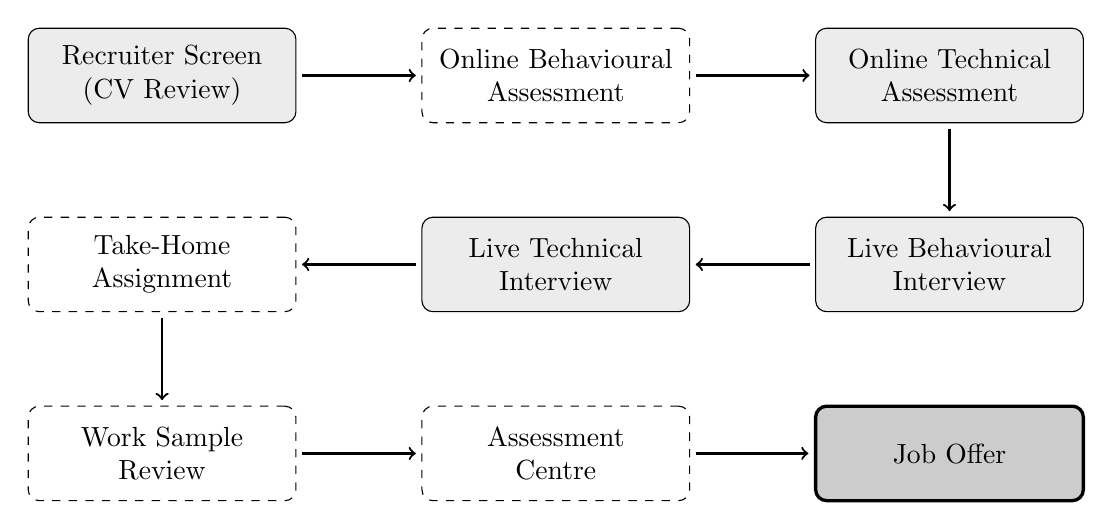
\begin{tikzpicture}[
    box/.style={
        draw,
        rectangle,
        rounded corners,
        align=center,
        minimum height=1.2cm,
        minimum width=3.4cm
    },
    core/.style={box, fill=gray!15},
    optional/.style={box, dashed},
    outcome/.style={
        box,
        fill=gray!40,
        draw=black,
        line width=1.2pt
    },
    arrow/.style={->, thick, shorten >=2pt, shorten <=2pt}
]

% ===== Row 1 =====
\node[core]     (cv)   at (0,0)   {Recruiter Screen\\(CV Review)};
\node[optional] (beh)  at (5,0)   {Online Behavioural\\Assessment};
\node[core]     (oa)   at (10,0)  {Online Technical\\Assessment};

% ===== Row 2 =====
\node[optional] (takehome) at (0,-2.4) {Take-Home\\Assignment};
\node[core] (techint) at (5,-2.4) {Live Technical\\Interview};
\node[core]     (live) at (10,-2.4) {Live Behavioural\\Interview};

% ===== Row 3 =====
\node[optional] (ac)    at (0,-4.8) {Work Sample\\Review};
\node[optional] (behint) at (5,-4.8) {Assessment\\Centre};
\node[outcome]  (offer) at (10,-4.8) {Job Offer};

% ===== Row 1 Arrows =====
\draw[arrow] (cv.east) -- (beh.west);
\draw[arrow] (beh.east) -- (oa.west);
\draw[arrow] (oa.south) -- (live.north);

% ===== Row 2 Arrows =====
\draw[arrow] (live.west) -- (techint.east);
\draw[arrow] (techint.west) -- (takehome.east);
\draw[arrow] (takehome.south) -- (ac.north);


% ===== Row 3 Arrows =====
\draw[arrow] (ac.east) -- (behint.west);
\draw[arrow] (behint.east) -- (offer.west);

\end{tikzpicture}
\caption[Technical recruitment pipeline]{Typical technical recruitment pipeline (core vs.\ optional stages).}
\label{fig:tech-recruitment-pipeline}
\end{figure}

When it comes to the application for technical positions, candidates will typically progress through multiple evaluation stages. 
While the sequence and steps taken often vary due to organisation size and maturity, industry research consistently shows that the technical recruitment pipelines will follow a multi-step structure \cite{cappelli2019}. 


\subsubsection{Recruiter Screen}
The hiring process for most organisations often starts off with a brief review of a candidate's CV to filter out 
candidates that are not suitable for the role. This is often performed by a recruiter or a hiring manager.
There has been a recent shift towards AI-driven pre-screening due to the rise in candidate applications, this
pre-screen is aimed to reduce the number of candidates that even make it to the first human review stage of the hiring process.
This significantly reduces applicant volumes, allowing for a more focused screening process, however, it is often at the cost
of algorithmic bias and opaque decision-making being introduced into the process.

Regardless of whether the process is a screen or a pre-screen, the CV itself is still the primary document evaluated.
However, industry research suggests that companies are becoming dissatisfied with typical CV data, such as past job titles
and educational prestige, when it comes to technical recruitment. It is noted that the industry is shifting towards skill-based
assessments to verify a candidate's competencies \cite{hackerrank2024skills}. Candidates are encouraged to provide their
GitHub URL as part of their application, however, research shows that this data is often reviewed inconsistently
during early stages, instead relying mainly on CVs as opposed to external behaviour evidence \cite{moore2023}.

\subsubsection{Online Behavioural Assessment} 
Larger enterprises commonly have an additional behavioural assessment, often in the form of a game, or a recorded interview, where candidates are prompted to record their response to common interview questions. 
Increasingly, these asynchronous video interviews are being augmented or fully driven by AI. Platforms employing machine learning 
algorithms can analyse a candidate's tone of voice, facial expressions, pacing, and keyword usage to algorithmically assess their 
personality and cultural fit. 
These tools, while uncommon in typical technical hiring pipelines, are more established in large-enterprise pre-screening: 
among Fortune 500 firms, 20\% already use asynchronous pre-recorded video interviews, with a further 17\% planning to adopt 
them, assessing dimensions such as communication style that are difficult to infer from a CV alone \cite{ithaka2018_assessment}. 
Smaller companies, however, rarely adopt such methods due to cost, limited perceived value and candidate-dropout risk.

\subsubsection{Online Technical Assessment}
Online technical assessments (commonly referred to as OAs) are core to the hiring process for many organisations. 
OAs often take place on platforms such as HackerRank and CodeSignal, and often focus on Data Structures and Algorithms (DSA). 
Industry surveys show that online technical assessments remain central to hiring pipelines: CoderPad's 2025 survey reports 
that 24.5\% of employers use asynchronous technical tests and 49.8\% use live coding interviews \cite{coderpad2025techhiring}, 
and CodeSignal highlights continued growth in standardised early-stage technical evaluations \cite{codesignal2023}.

\subsubsection{Live Behavioural Interview}
Live behavioural interviews are a common stage in technical recruitment, often conducted by HR or hiring managers to assess a candidate's cultural fit, communication skills and motivations for the role and company.
This process follows traditional interview formats, with a focus on behavioural questions alongside further discussions regarding the candidate's background, providing a better insight into a candidate's previous experiences and soft skills.

\subsubsection{Live Technical Interview}
Live technical interviews refer to the group of assessments which often involve an element of programming in front of an engineer at the hiring organisation, often involving live-coding, pair programming, or on-the-spot problem solving. 
These forms of assessment remain as a core part of the process for most software engineering hiring processes when it comes to evaluating a candidate's technical proficiency. 
As such, many organisations treat this as a central evaluation stage. 
While reliable aggregate data for this is scarce, multiple industry-level reports and practitioner accounts can confirm that live technical interviews remain an essential method for assessing candidates \cite{karat2020}. 

Some academic and industry critiques point out the limitations of this format, specifically stress under observation, lack of realism, and poor predictive validity for long-term developer performance. 
This suggests that hiring pipelines should leverage alternative assessment methods as opposed to solely live coding rounds \cite{behroozi2019hiring}.

\subsubsection{Take Home Assignment}
For organisations that prefer “skill-based hiring”, they may incorporate take-home tests as part of their technical hiring process. 
These assignments require a candidate to build or extend a small system, followed by a review interview. 
According to TestGorilla's 2024 survey, a large portion of employers report using assignment, or work-sample based assessments as a part of their hiring pipeline, highlighting the relevance of take-home assessments for a realistic evaluation of coding ability and design choices \cite{testgorilla2024}. 
They argue that these assignments provide a better benchmark for the candidate's real-world development skills rather than time-limited algorithmic tests and whiteboard interviews.

\subsubsection{Work Sample Review}
Many employers like to also use real-world evidence, such as GitHub repositories, open-source commits and portfolio projects to assess a candidate's ability to build software. 
This data is often a critical differentiator, as it is able to separate a candidate's claims from their actual abilities.
Historical data highlight that the majority of firms (80\% of small and 66\% of large firms) place high value on portfolio evidence,
such as GitHub \cite{hackerrank2018skills}. Recent reports also come to a similar conclusion, that verified technical 
assessments are essential in addressing the limitations of traditional CVs \cite{hackerrank2024skills}.
However, this is often done later in the pipeline due to the time and expertise required for evaluation. 
Academic literature shows that work-sample tests are one of the highest-validity predictors of job performance (validity coefficient of 0.54) \cite{schmidt1998}, significantly outperforming CV-based assessments.

\subsubsection{Assessment Centre}
An assessment centre (commonly referred to as AC) is a structured multi-exercise evaluation process, often used in graduate programs and enterprise-level hiring. 
Recent UK survey data suggest that a minority of organisations (32\% in 2020) use formal assessment centres as part of their selection process \cite{cipd2020_resourcing}. 
Where assessment centres are used, UK employers commonly apply methods such as group exercises, psychometric tests, role plays and combined tasks to evaluate teamwork, communication and problem-solving \cite{cipd2022}. 
While not widely used, ACs remain useful for gaining deeper insights into the candidate's interpersonal and non-technical capabilities.

\subsubsection{Relevance to MERIT}
Given the complexities and inconsistencies that are present in the technical hiring process, the screening stage remains to be the most influential, yet error prone point in the process. 
Organisations rely heavily on this filter, yet early decisions are often solely based on a brief CV review, which is often shown to be vulnerable to bias, information loss and unreliable judgement. 
MERIT will target this part of the pipeline to improve accuracy, fairness and evidence-quality in order to produce the greatest organisational impact.

MERIT will strengthen screening through the integration of multi-source evidence, such as GitHub activity, CV data, and other sources, to provide verifiable behavioural and technical indicators. 
This early-stage assessment can reduce or refine the need for later steps, such as online coding tests, manual work-sample reviews, and broad behavioural screens, while still highlighting areas where further evaluation is necessary. 
The system will be designed to be adaptable across different organisation sizes, for example smaller firms will benefit from reduced reliance on time-consuming take-home tasks, and larger firms can improve their structured assessments with transparent data-driven insights. 
By transforming the earliest decision point into a more reliable and insightful stage, MERIT helps to create a fairer, more consistent and efficient technical hiring process.


\section{Data Sources}
\label{sec:data-sources}
Technical recruitment often requires multiple data sources to be provided to evaluate candidates beyond traditional CVs, but these are rarely used in practice. These sources have the potential to provide insights into the extensive professional history, technical competencies, behavioural tendencies as well as real-world coding practices. Effective multi-source screening will require a deeper understanding of the strengths and limitations of these data channels.


\begin{table}[htbp]
    \centering
    \caption[Overview of supplementary recruitment data sources]{An overview of supplementary data sources, their value to technical recruitment, and their inclusion in MERIT.}
    \label{tab:data-sources}
    \small
    \renewcommand{\arraystretch}{1.4}
    \begin{tabularx}{\textwidth}{>{\raggedright\arraybackslash\bfseries}p{2.6cm} >{\raggedright\arraybackslash}p{3.2cm} >{\raggedright\arraybackslash}X >{\centering\arraybackslash}p{1.5cm}}
        \hline
        \textbf{Data Source} & \textbf{Primary Function} & \textbf{Value to Technical Recruitment} & \textbf{Included?} \\ \hline
        Curriculum Vitae (CV) & Self-reported professional summary & Baseline for initial screening. Highly vulnerable to embellishment and self-report bias \cite{henle2019_resume_fraud,dunning2004}. & Yes \\
        GitHub & Version-controlled code repositories & Richest source of verifiable work-sample evidence. Demonstrates tech stack usage and coding style \cite{hackerrank2018skills,hackerrank2024skills}. & Yes \\
        LinkedIn & Professional identity and networking & Expands upon CV details. Used by 72\% of recruiters \cite{jobvite2020}. & Yes \\
        LeetCode \& HackerRank & Algorithmic practice and live assessments & Demonstrates tested technical ability and problem-solving under constraints \cite{coderpad2025techhiring}. & No \\
        Stack Overflow & Software engineering Q\&A exchange & Highlights communication style, community engagement, and domain specialisation \cite{vasilescu2013}. & No \\
        Social Media & General personal networking & Used for background checks to identify ``red flags'' \cite{careerbuilder2017_social}. High risk of bias (Note: excludes LinkedIn). & No \\ \hline
    \end{tabularx}
\end{table}

\subsubsection{Relevance to MERIT}
As shown above, there are a variety of external data sources that can be used to evaluate a candidate's suitability for a technical role
beyond the traditional Curriculum Vitae (CV). Being able to capture and integrate multiple data sources can help provide more factors
to differentiate between candidates, allowing for a more comprehensive view of a candidate's suitability for a role. MERIT aims to 
integrate GitHub as a supplementary data source due to it serving as a strong indicator of a candidate's technical ability. LinkedIn
will also be selected as a strong indicator of a candidate's professional experience and also to account for errors in the CV parsing process.
Other data sources such as LeetCode and HackerRank are likely to not be selected as supplementary data sources due to the time 
constraints during development, however, they are still considered as potential future data sources for MERIT.




\section{Manual Screening}
In smaller organisations, early-stage screening is still likely to be manually conducted, 
due to the cost of implementing and maintaining an automated screening system.
Recruiters and hiring managers will usually review a candidate's CV, along 
with application data, to compare against the job description to determine 
whether the applicant meets the minimum experience and skill requirements.
The screening stage is designed not to find the best candidate, 
but to instead to reject candidates that are considered unsuitable for the role, 
allowing for a more focused and efficient interview process.
In order to manage large applicant pools, recruiters may also introduce 
implicit filtering criteria in an attempt to simply reduce the number of 
candidates progressing into more resource-intensive interview stages.
While manual screening can be effective in recruitment, it often suffers 
from a range of limitations and biases that can reduce the overall quality, 
fairness and consistency of the process.

A primary issue revolves around biases due to time pressure and superficial 
evaluation, as recruiters usually spend little time on a first-pass, leading 
to them overlooking critical information.
The issues are further exacerbated by information overload and cognitive load 
bias, where excessive information leads to increased decision difficulties as 
well as a reliance on cognitive shortcuts rather than careful evaluation, as shown in research on information overload \cite{che2019}.
Furthermore, the repetitive task and fatigue effect suggests that when recruiters 
process multiple candidates in a session, their decision quality degrades.
This is supported by a PNAS study from Danziger et al., which highlights that favourable rulings drop 
sharply as decision-makers process more cases without breaks \cite{danziger2011}. 
Note that this work studied judicial parole decisions rather than hiring, but the same fatigue pattern may also apply to high-volume CV screening.
The mood and emotional state bias causes further issues as the Affect Infusion 
Model indicates that a recruiter's emotional state under stress can lead to a change 
in their perception or judgement of a candidate's suitability for that role \cite{forgas1995}.

Beyond these operational constraints, the screening process is also influenced by 
other distortions that introduce further bias.
The determinism of the recruitment process is affected by the contrast effect, as 
candidate evaluation may be unfairly affected by the quality of candidates that precede 
them \cite{palmer2014}.
This issue is made worse with the anchoring bias, where they over-rely on the first 
piece of information encountered, such as a previous employer or job title, which then 
disproportionately influences the rest of the screening \cite{buijsrogge2021}.
Halo and horn effects also tie in closely to this, where a recruiter generalises from 
one positive or negative attribute, such as a prestigious company, or a single typo, to 
the entire candidate profile \cite{thorndike1920}.
The previously mentioned issues are further worsened due to imperfect and exaggerated 
self-reported information where candidates may embellish or misrepresent their skills and 
experiences to appear more favourable \cite{dunning2004}.

Finally, manual screening is also vulnerable to systemic discrimination and group-based preferences.
For instance, field experiments by Bertrand and Mullainathan found that name 
and ethnic discrimination plays a key issue.
This is shown through their findings where “white sounding” names received around 
50\% more callbacks compared to “African American sounding” names despite identical qualifications \cite{bertrand2004}.
The main cause of this often comes down to similarity bias and in-group bias. This is the idea that
individuals tend to favour applicants who resemble them, often in terms of factors such as background, nationality
and educational route \cite{tajfel1986}.


The core limitations, as shown above, come down to time pressure, cognitive load, and applicant volume. 
The biases mentioned uncover the unfairness behind manual screening, more specifically the lack of consistency
and objectivity in this process.
As more candidates enter the application process, these psychological and procedural 
limitations compound further, leading to inconsistent outcomes, reduced fairness and 
also the potential for a poor selection quality.
Such challenges highlight the need for a more reliable, systematic and transparent 
screening method, more specifically automated, data-driven systems that are able to 
evaluate a candidate against a job requirement with better consistency, scalability, 
and a reduced vulnerability towards any potential human bias.

